\section{Napájení}
\label{nabijecka}
Jako napájení celého trezoru slouží dvě li-on baterie 18650 každá o uváděné kapacitě 3400 mAh. 
Dva tyto články tak poskytují BlackBoxu dostatek energie na 32 hodin provozu se spuštěným světelným kruhem v módu DarkMode \ref{WS2812}.
Napětí článků však nevyhovuje potřebám trezoru, a~tak je na trezoru lineární 
stabilizátor \href{https://datasheet.lcsc.com/szlcsc/1808280153_STMicroelectronics-LD39200PU33R_C222192.pdf}{NCP708} \parencite{ld39200}, 
který zajišťuje napětí 3,3~V pro většinu systému. Kromě LD39200 je zde také step-up \href{https://datasheet.lcsc.com/szlcsc/Feeling-Tech-FP6276AXR-G1_C83308.pdf}{FP6276} \parencite{fp6276a}, 
který zajišťuje napájení 5~V sloužící primárně pro LED WS2812 a~v~druhé řadě napájí motor zámku.
Zapojení stabilizátoru a step-upu je přiloženo na obrázku v příloze \obr{fig:E4-sch_zdroj}.

\begin{figure}[h]
    \centering
    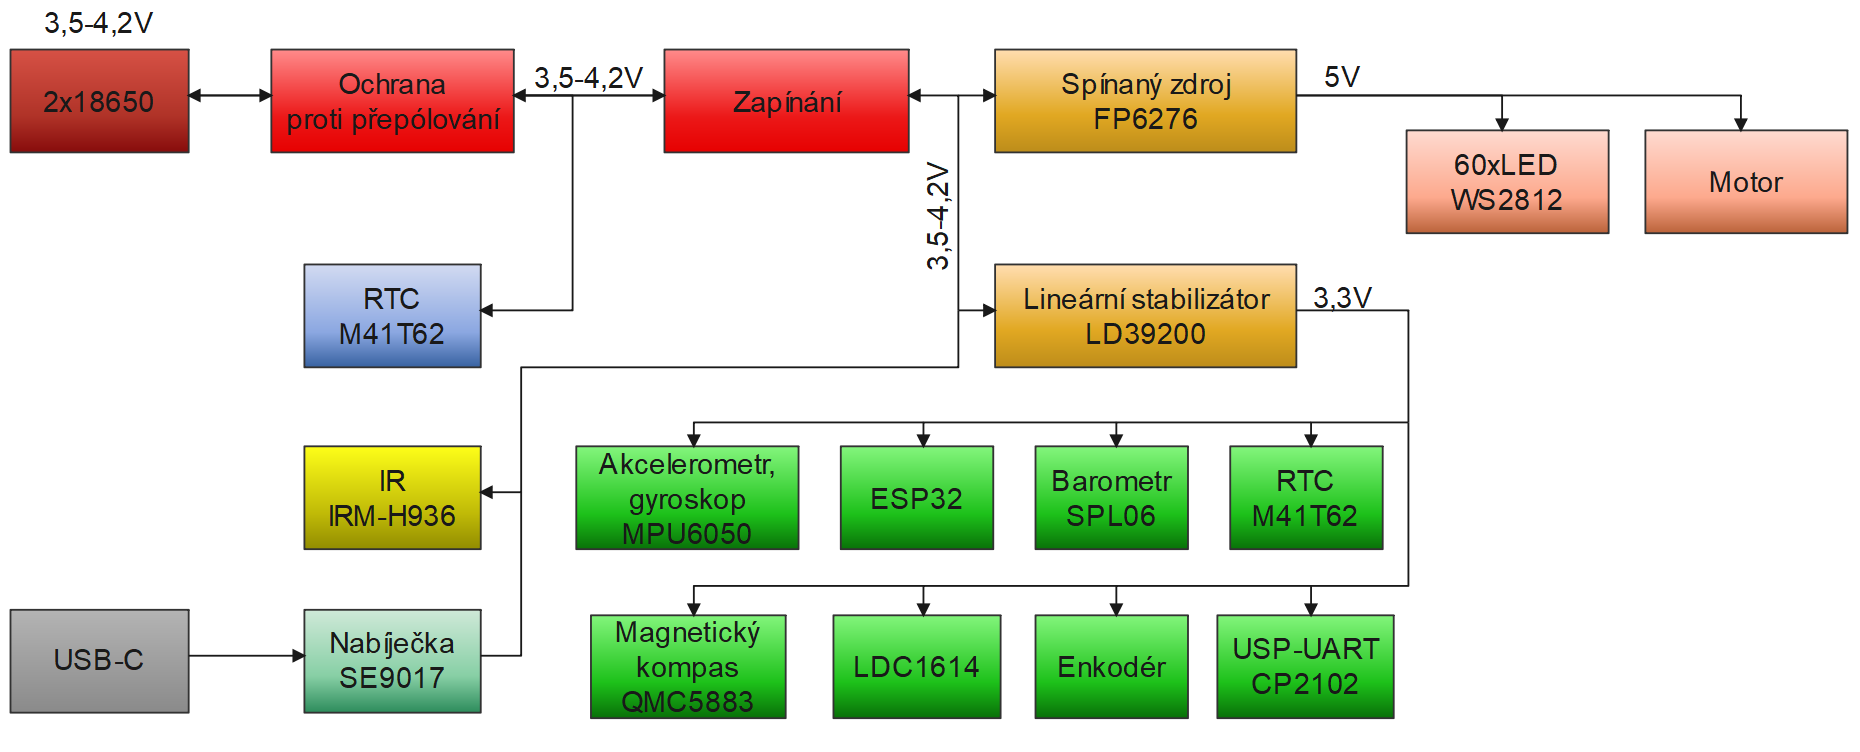
\includegraphics[width=\textwidth]{kapitoly/obrazky/E4/napajeni/napajeni.png}
    \caption{Blokové schéma rozvržení napájení}
    \label{fig:E4-napajeni}
\end{figure}

\newpage
\paragraph*{Zapínání}
\addcontentsline{toc}{paragraph}{Zapínání}
Aby se trezor mohl vypnout a~tak šetřit energii, je vybaven obvodem, který to umožňuje \obr{fig:E4-zapinani}.

Při připojení článků se napětí dostane nejprve na PTC\footnote{polymerová PTC, vratná pojistka } \parencite{polyfuse},
které slouží jako ochrana proti nadproudu, například v případě, kdy uživatel připojí dva různě nabité články nebo jeden z~nich přepóluje.
Pokud se proud dostane skrz PTC, dostane se na tranzistor Q11 \parencite{power_MOSFET}, skrz který projde, jen pokud jsou články správně pólovány.
Když se napětí dostane přes ochranu proti přepólování, dostane se na 
vývod source
tranzistoru Q5 \parencite{power_MOSFET}, skrz R6 na vývod drain
Q1 a~pak skrz R7 na obě strany C61.
Pokud v~takovéto situaci dojde ke~stisku SW3, projde zem skrz C61 na vývod gate tranzistoru Q5. 
V~tu~chvíli se Q5 otevře na dostatečně dlouhou dobu, 
aby naběhla třívoltová větev a~skrz pull-up\footnote{Na obrázku \obr{fig:E4-zapinani} vpravo je jen poznámka, reálná součástka je ve schématu společně s ESP32 na obrázku \obr{fig:E4-sch_ESP32}.}
se zvedlo napětí na gate tranzistoru Q1 na téměř 3,3~V. Q1 se tak otevře a~už~trvale připojí GND na gate tranzistoru Q5, trezor se tak zapne. Pokud v takové chvíli procesor stáhne dráhu SHUTDOWN 3V3-5V 
na GND, nebo dojde ke stisku SW5, opět se uzavře Q1 a~skrz R6 projde na gate Q5 napětí, které Q5 uzavře a~tak elektroniku opět vypne.

\begin{figure}[h]
    \centering
    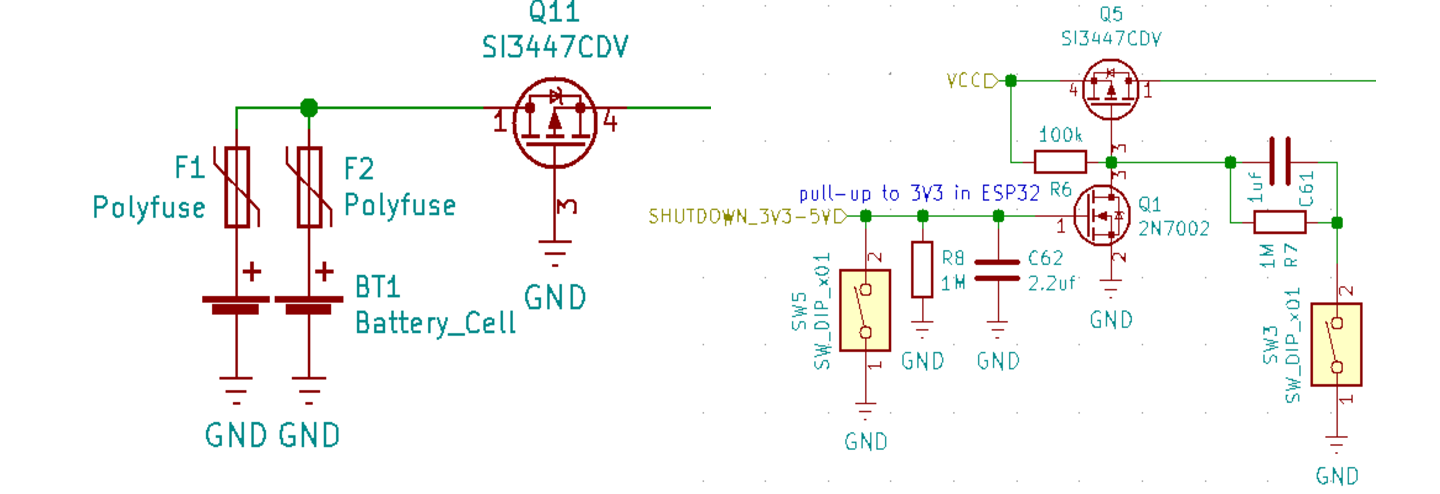
\includegraphics[width=\textwidth]{kapitoly/obrazky/E4/napajeni/ochrana_proti_prepolovani_a_zapinani.png}
    \caption{Ochrana proti přepólovaní a zapínání}
    \label{fig:E4-zapinani}
\end{figure}



\paragraph*{Step-up vysvětlení funkce}
Zapojení step-upu\footnote{Spínaný zdroj, který spíná vstupní napětí na vyšší napětí.} je~o~něco složitější než zapojení stabilizátoru, 
který stačí připojit a funguje. 
Spínané zdroje využívají ke své funkci cívku, na které vzniká změna napětí. Proud cívkou se nedá okamžitě zastavit a právě toho se využívá. 
Když se cívka připne mezi napájení a zem, začne skrz ní tést prod. V okamžiku, kdy se pak jedna strana cívky odpojí od zdroje, 
musí se stále tekoucí proud kompenzovat změnou napětí.
Takže ve chvíli, kdy se cívka odpojí od záporného pólu vzroste na této straně cívky napětí. 
Jak moc napětí stoupne se pak odvíjí od velikosti proudu, který skrz cívku před odpojením tekl.

\vspace{-5mm}

\paragraph*{Step-up zapojení na desce trezoru} Pro ovládání spínání step-upu jsem zvolil \href{https://datasheet.lcsc.com/szlcsc/Feeling-Tech-FP6276AXR-G1_C83308.pdf}{FP6276}.
Tento obvod jsem si vybral, protože mi vyhovoval jak po stránce napětí, tak po~stránce efektivity a~ceny a~zároveň byl v~nabídce firmy JLCPCB.\footnote{Firma, u~které jsem desky vyráběl a~osazoval.}
Obvod jsem z~většiny zapojil dle doporučení výrobce, mojí prací bylo vlastně jen správně určit hodnoty 
jednotlivých součástek. Na ovládání pinu EN, který FP6276 vypíná, jsem připojil pull-up k napájení a~pro možnost step-up vypnout tranzistor Q2 \parencite{cj3134k}. 
Pokud tedy procesor stáhne dráhu SHUTDOWN 5V k zemi, a~tak přivede na gate tranzistoru Q2 zem, 
Q2 se zavře. Tím se na pin EN přivede skrz R18 napájecí napětí, které step-up spustí. 
Pokud se na gate Q2 přivede naopak logická jedna, Q2 se~otevře a~na~EN~se~dostane zem, která naopak provoz step-upu zastaví.
\vspace{-5mm}
\begin{figure}[h]
    \centering
    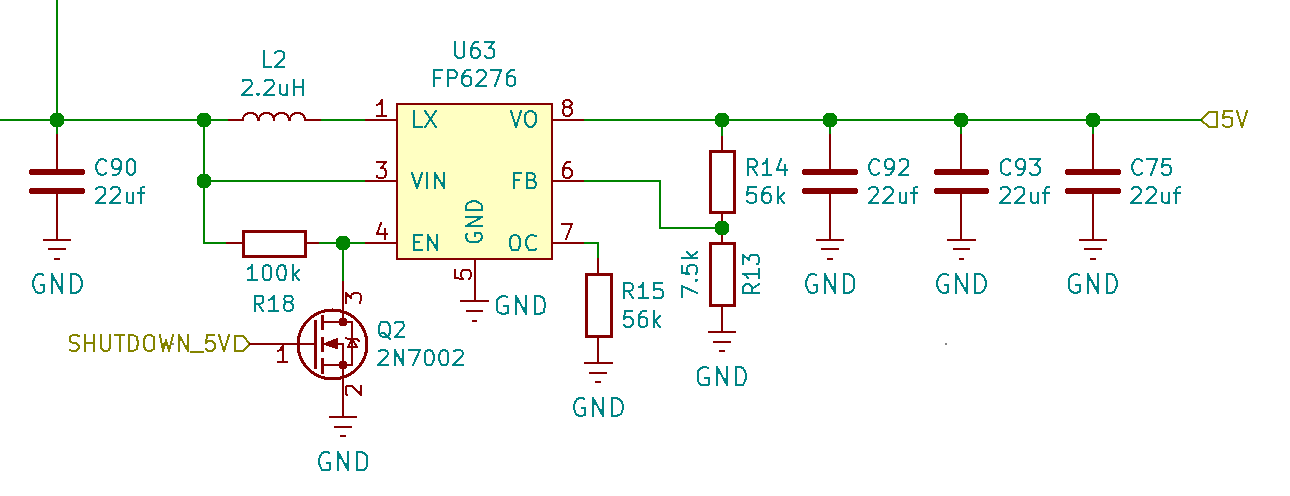
\includegraphics[width=0.9\textwidth]{kapitoly/obrazky/E4/napajeni/step-up.png}
    \caption{Zapojení step-upu}
    \label{fig:E4-step-up}
\end{figure}

\paragraph*{Stabilizátor}
\addcontentsline{toc}{paragraph}{Stabilizátor}

Stabilizátor \href{https://datasheet.lcsc.com/szlcsc/1808280153_STMicroelectronics-LD39200PU33R_C222192.pdf}{LD39200} \parencite{ld39200} má pin EN, který slouží k~je\-ho vypínání. 
Pokud je na nem logická 0, je~stabilizátor vypnut a~pokud 1, je zapnut. Vzhledem k~tomu, že v~mém zapojení toto vypínaní nepotřebuji, je pin EN připojen 
přes R10 přímo na napájecí napětí, a~tak je stabilizátor trvale zapnut.
Konkrétně LD39200 jsem vybral kvůli malému pádu napětí, který vyžaduje pro svůj provoz, typicky 120~mV při proudu 1~A. Vzhledem k~tomu, že~na~vstupu 
mám maximálně 4,2~V, tak maximální napěťový pád, který mám k~dispozici, je~0,9~V, protože na výstupu požaduji napětí 3,3~V. Navíc musím počítat 
i~s~vybitou baterií, u~které počítám s~napětím 3,5~V. %Rád bych počítal s~napětím ještě nižším, ale v~nabídce JLCPCB jsem nenašel stabilizátor s~nižším pádem napětí a~zároveň dostatečným proudem.

\begin{figure}[h]
    \centering
    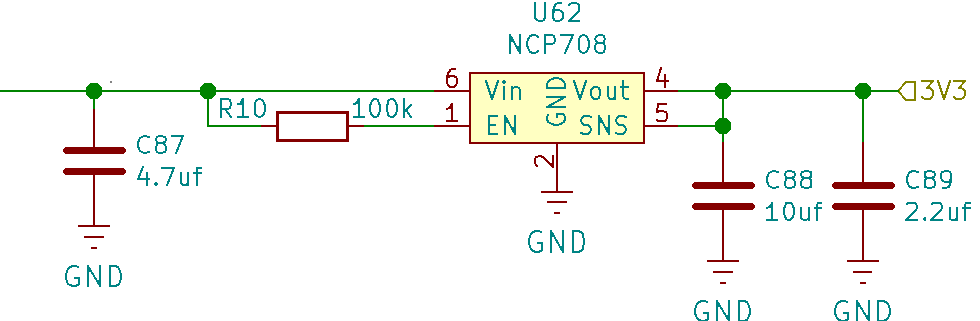
\includegraphics[width=0.9\textwidth]{kapitoly/obrazky/E4/napajeni/stabilizator.png}
    \caption{Zapojení stabilizátoru}
    \label{fig:E4-stabilizator}
\end{figure}

\newpage

\paragraph*{Měření napětí baterií}
\addcontentsline{toc}{paragraph}{měření napětí baterek}

\begin{wrapfigure}{R}{0.4\textwidth}
    \centering
    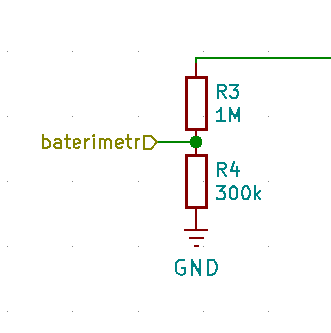
\includegraphics[width=0.4\textwidth]{kapitoly/obrazky/E4/napajeni/delic_baterimetru.png}
    \caption{Měření napětí baterií\label{fig:baterimetr}}
\end{wrapfigure}

Aby trezor mohl zjistit, že má vybité baterie, musí mít možnost jim měřit napětí. ESP32 obsahuje AD převodník, takže není problém měřit napětí baterie 
i poměrně přesně. Kde však problem nastává, je maximální napětí, které je schopen měřit, a~to 1,1~V. ESP32 má možnost připojit k~AD převodníku dělič,
aby se~na~pin dalo přivést napětí až 3,3~V. To ale pořád není dostatečné, a~také se~tím snižuje přesnost měření. Proto je na desce jednoduchý dělič napětí
složený ze~dvou odporů, jednoho s~hodnotou 1~M$\Omega$ a~druhého 300~k$\Omega$, takže při plně nabitých bateriích bude na výstupu děliče 0,97~V. %todo kolik je tam těch baterek. <- nevim jak to tam teď elegantně dopsat a ani bych to nepovažoval za nějak zvlášť podstatnou informaci v odstavci o měření napětí, je to hned v první větě pod nadpisem napájení